\chapter{Introduction}
\label{sec:intro}

Molecular Dynamics (MD) is a computational method used to simulate the behavior of atoms and molecules over time. In recent years, MD simulations have become essential in many scientific fields, including chemistry, physics, biology, and materials science. Such simulations are used to study various systems, ranging from simple gases and liquids to complex biological molecules and new materials.

MD simulations act on an atomic level and attempt to explain macroscopic properties of a system from the interactions between the individual atoms and molecules. The recent advances in computational power have made it possible to simulate systems with millions of particles over long time scales, allowing researchers to study complex systems in unprecedented detail. Contrary to experimental methods, MD simulations can provide detailed information about the behavior of atoms and molecules, sometimes inaccessible to experimental methods~\cite{Perilla2017}.

Two illustrations of such simulations are shown in \autoref{fig:hiv_capsid} and \autoref{fig:md_simulation_loop}. The first image shows a simulation of the HIV-1 capsid, a protein shell that surrounds the genetic material of the human immunodeficiency virus (HIV). Using a simulation-based approach, researchers could study critical properties of the HIV-1 capsid, which would be difficult to access using other methods~\cite{Perilla2017}. The second image shows a simulation of shear band formation around a precipitate in metallic glass. This simulation found evidence that depending on the precipitate size, shear bands can either dissolve, wrap around, or be blocked by the precipitate~\cite{Brink2016}. This information is crucial for understanding the mechanical properties of metallic glasses and can be used to design new materials with improved properties.


\begin{multicols*}{2}
    \begin{figure}[H]
        \centering
        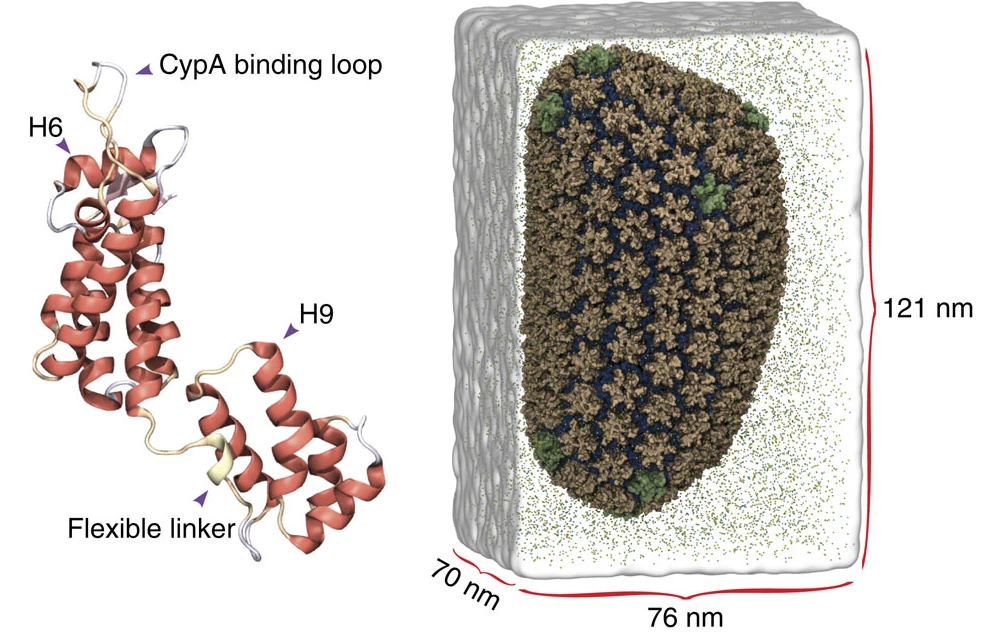
\includegraphics[width=0.9\columnwidth, trim={0cm 0 0cm 0cm}]{figures/Intro/HIV-1.png}
        \caption{MD simulation with 64,423,983 atoms of the HIV-1 capsid. Perilla et al.~\cite{Perilla2017} investigated properties of the HIV-1 capsid at an atomic resolution.}
        \label{fig:hiv_capsid}
    \end{figure}

    \begin{figure}[H]
        \centering
        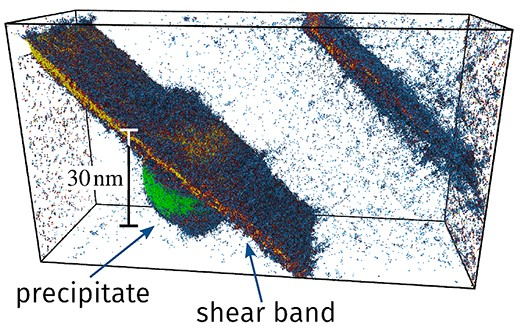
\includegraphics[width=0.9\columnwidth,trim={0cm 0 0cm 0cm}]{figures/Intro/metallic-glass-crack.jpg}
        \caption{MD simulations of shear band formation around a precipitate in metallic glass, as demonstrated by Brink et al.~\cite{Brink2016}.}
        \label{fig:md_simulation_loop}
    \end{figure}
\end{multicols*}

Simulating such systems is very computationally demanding and typically requires the use of high-performance computing (HPC) systems for large-scale simulations. Another challenge is the development of efficient simulation software that can handle the complexity of the systems and make optimal use of the available computational resources. This thesis focuses on the development of AutoPas, a high-performance, auto-tuned particle simulation library for many-body systems, which tries to address these challenges by dynamically switching between algorithms and data structures to guarantee high performance throughout the simulation.

This switching mechanism is guided by so-called \textit{tuning strategies}, which are responsible for exploring the space of available algorithms and data structures and attempt to find appropriate configurations for the current simulation state. The development of efficient tuning strategies is crucial, as efficient choices can significantly reduce the runtime of the simulation, making MD simulations more accessible to researchers and enabling the study of more complex systems.

This thesis focuses on the development of a novel fuzzy logic-based tuning strategy for AutoPas, which allows users to encode their domain knowledge in the tuning process. Furthermore, we investigate a data-driven approach to automatically generate fuzzy systems, and we will show that the proposed fuzzy tuning strategy can outperform existing tuning strategies on specific benchmarks.